\chapter{Molten Salt Reactor Modeling}% \label{cha:msr_modeling}
%% lit review goes here
Much of our knowledge about \Gls{msr}s come from experiments on a test reactor
called the \Gls{msre} conducted at \Gls{ornl} in the 1960s, which demonstrated
the viability of the \Gls{msr} concept for use in civilian power programs
\cite{haubenreich_experience_1970} \cite{rosenthal_molten-salt_1970}. The \Gls{msre} reactor to this day remains one of the few \Gls{msr}s to operate.
%% Maybe briefly mention other historical MSRs?

As of writing this thesis, there are no \Gls{msr}s currently in operation; we
must rely on computational and/or surrogate models to further study \Gls{msr}
physics. The \Gls{msre} is a popular choice for computational models due to the
availability of experimental data to compare results against. For example,
Roelofs et al used the system thermal hydraulics code SPECTRA to model steady
state parameters of the fuel-salt, \Gls{dnp} drift, and various fission product
behaviors in comparison with actual MSRE data \cite{roelofs_molten_2021}.
Podila et al performed a \Gls{cfd} simulation of the \Gls{msre} core to
investigate the ability of \Gls{cfd} to predict 3D effects in this kind of
reactor \cite{podila_cfd_2019}. 
%cite some MSRE studies
In addition to the \Gls{msre}, the \Gls{msfr} \cite{merle-lucotte_launching_2011}
and \Gls{msbr} \cite{robertson_conceptual_1971} conceptual reactors are well
developed and are actively used in research. Park et al performed a whole core
analysis of the \Gls{msbr} using \MCNPSIX with additional depletion and
reprocessing using \CINDERNINETY and a custom Python script \cite{park_whole_2015}.
Aufiero et al extended \SerpentTWO with online fuel reprocessing capabilities to
study depletion in the \Gls{msfr} \cite{aufiero_extended_2013}. These efforts
illustrate that \Gls{msr} modeling encompasses a wide range of physics domains.

\section{Modeling depletion in MSRs} Recall in Sections
\ref{sec:molten_salt_reactors} and \ref{sec:msr_codes} we introduced the
concepts of fuel depletion and removal and feed processes, and we established
the importance of modeling fuel depletion to \Gls{msr} licensing. Depletion
simulations on \Gls{msr}s are difficult to verify through direct
measurement due to the lack of a physically operating reactor. Even so,
simulations will give us a good idea of what kinds of nuclides we can expect to
show up. Table \ref{tab:msr_depletion_tools} summarizes some currently available
software tools that can model depletion in \Gls{msr}s. 

\begin{table}[htpb] 
    \centering 
    \caption{Software tools that can model \Gls{msr} depletion with fuel reprocessing} 
    \label{tab:msr_depletion_tools}
    \begin{tabulary}{\linewidth}{|C|C|C|C|} 
        \hline
        Software tool & Description & Reprocessing scheme & Citation\\
        \hline 
        \ADDER & Interface code with internal depletion capabilities & Component-based continuous & \cite{nelson_molten_2021}\\
        \hline
        \SCALE & Suite code & Continuous & \cite{betzler_molten_2019}\\
        \hline 
        \SaltProc & Interface code & Component-based batch-wise & \cite{rykhlevskii_saltproc_2018}\\
        \hline 
        \SerpentTWO & Transport code with internal depletion capabilities & Material or universe based continuous & \cite{aufiero_extended_2013}\\
        \hline
    \end{tabulary}
\end{table}

\SaltProc has been used to perform lifetime depletion analysis on full-core
models of the \Gls{msbr} \cite{rykhlevskii_modeling_2019} and the Transatomic
Power \Gls{msr} \cite{rykhlevskii_fuel_2020}. As seen in Figure
\ref{fig:msbr_spectrum_comp}, the BOL and EOL neutron flux spectra for the MSBR
results qualitatively matches those reported Park et. al \cite{park_whole_2015},
as well as with data from the original MSBR report from Robertson et. al
\cite{robertson_conceptual_1971}.

\begin{figure}[!htpb]
    \centering
    \subfloat[][]{
        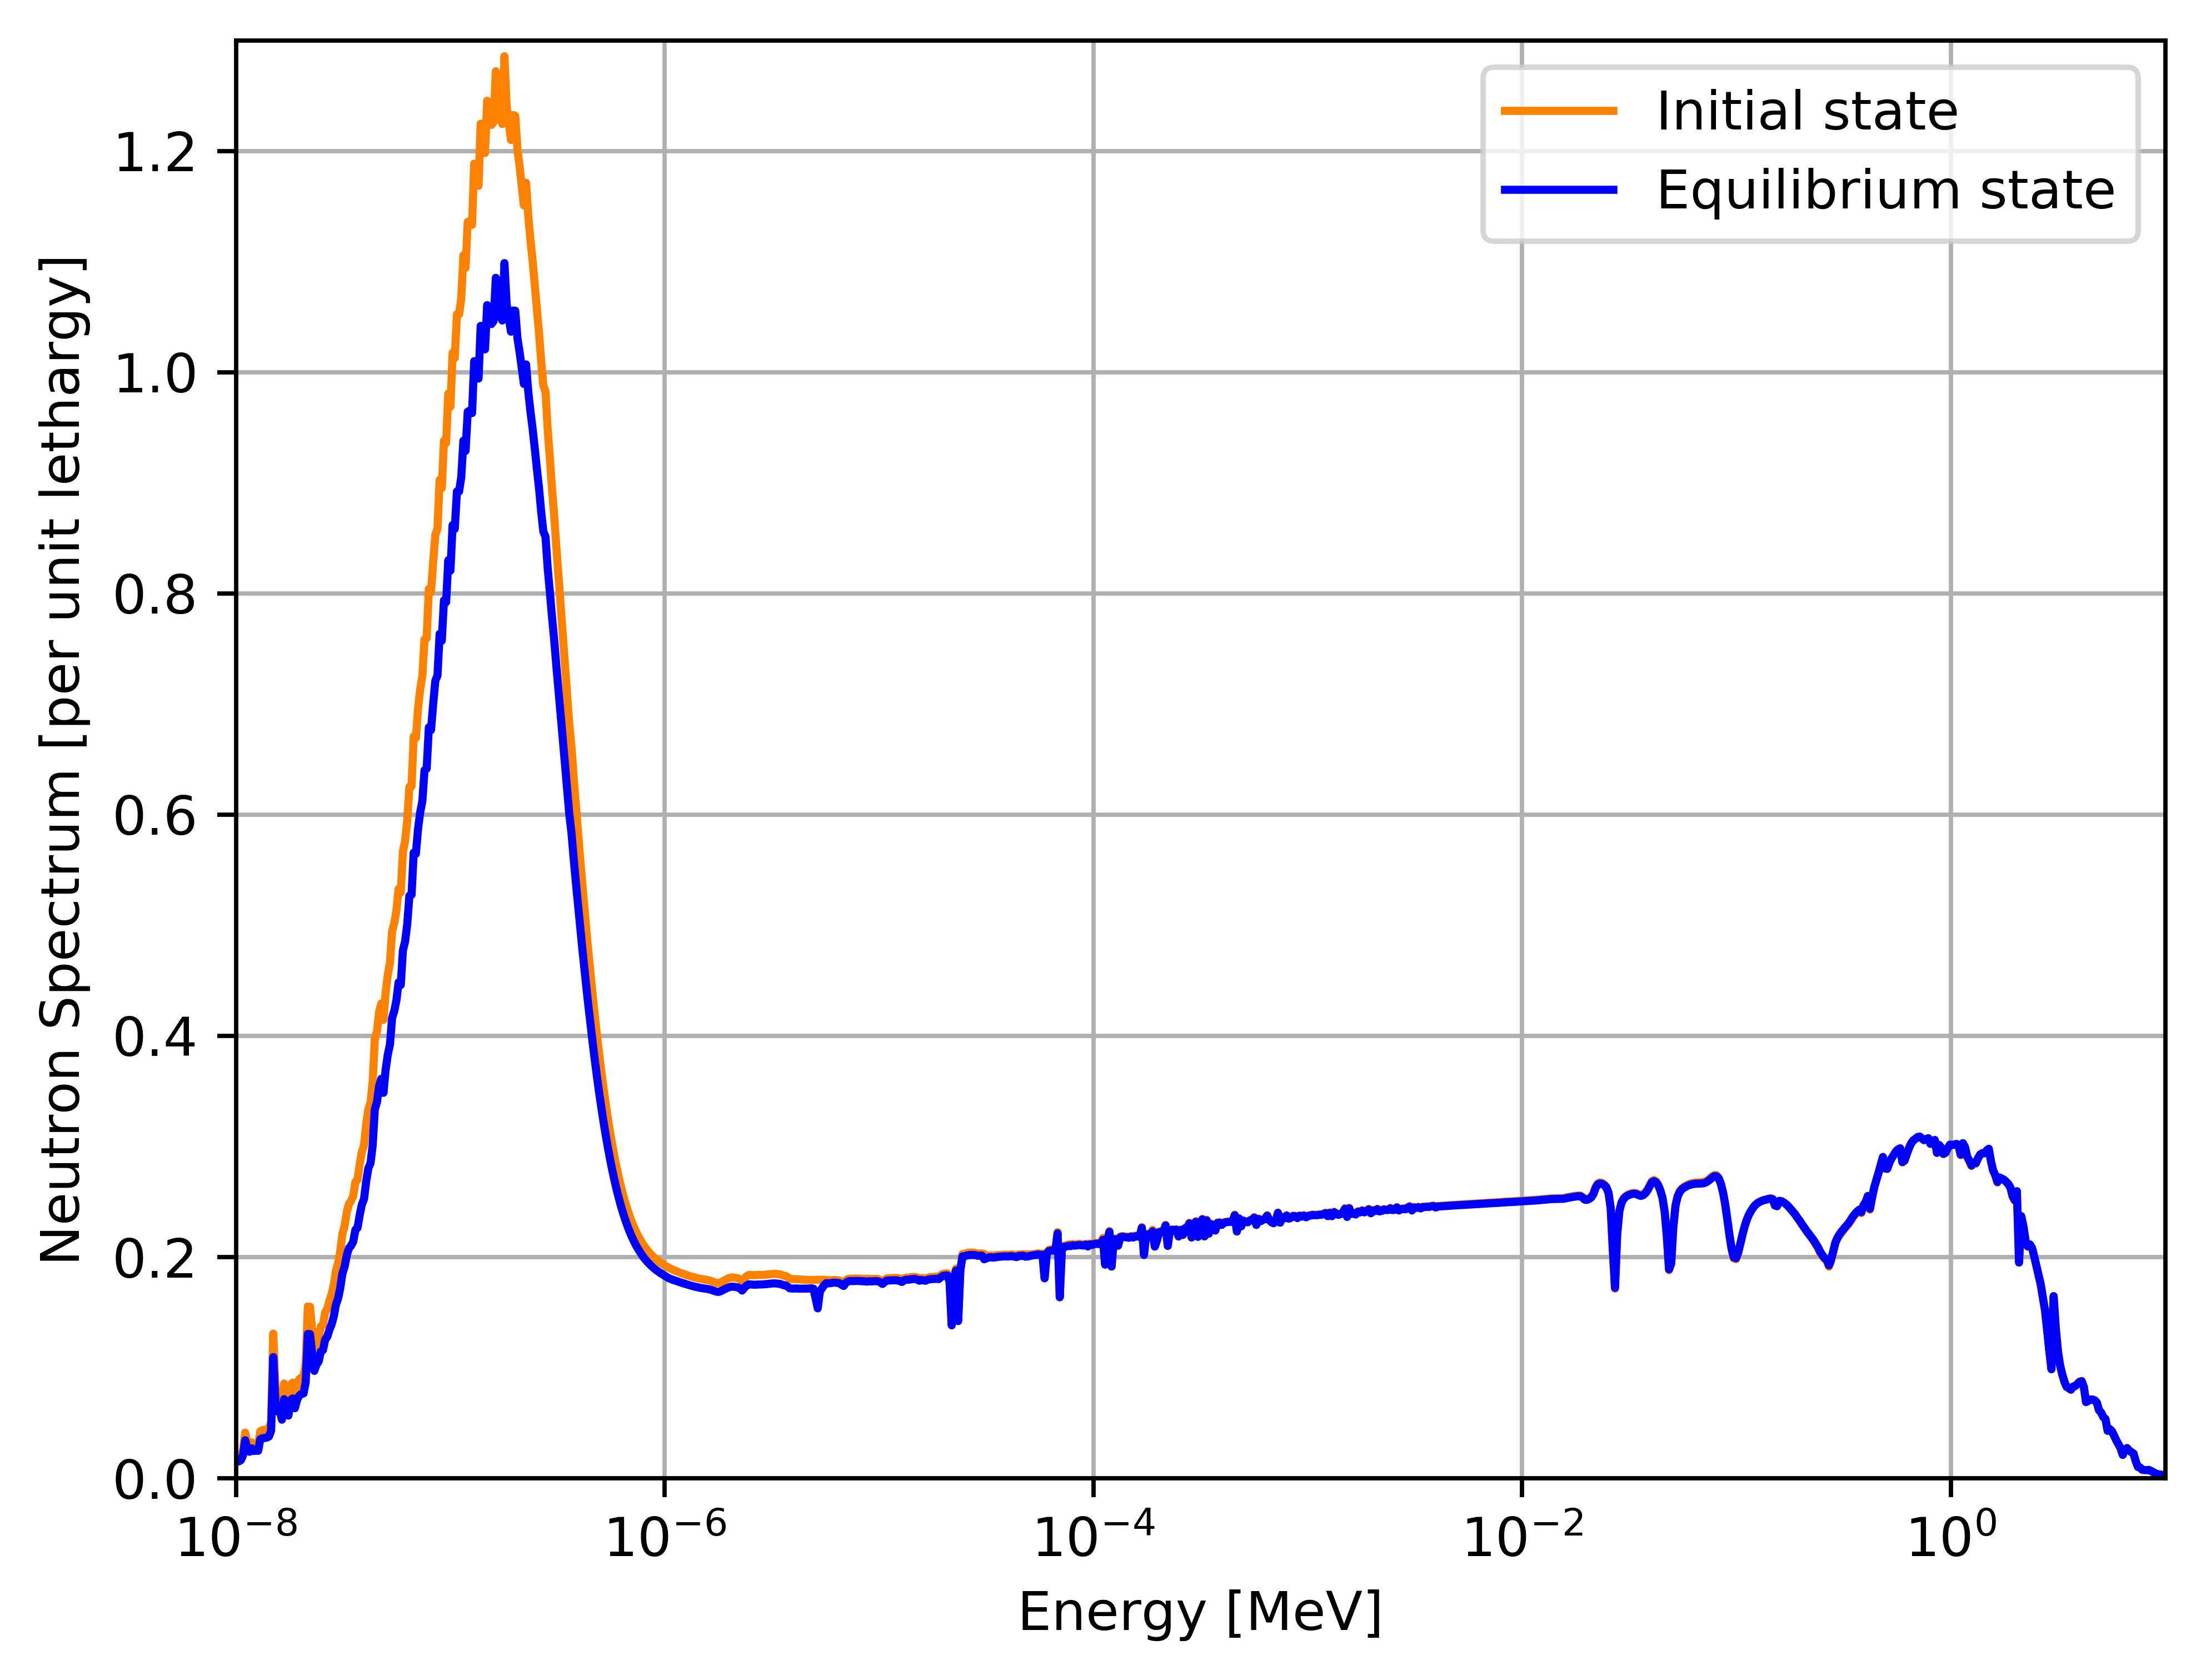
\includegraphics[width=0.5\linewidth]{figs/ch2/msbr_spectrum-rykhlevskii.png}
        \label{fig:msbr_spectrum_sub1}
    }
    \subfloat[][]{
        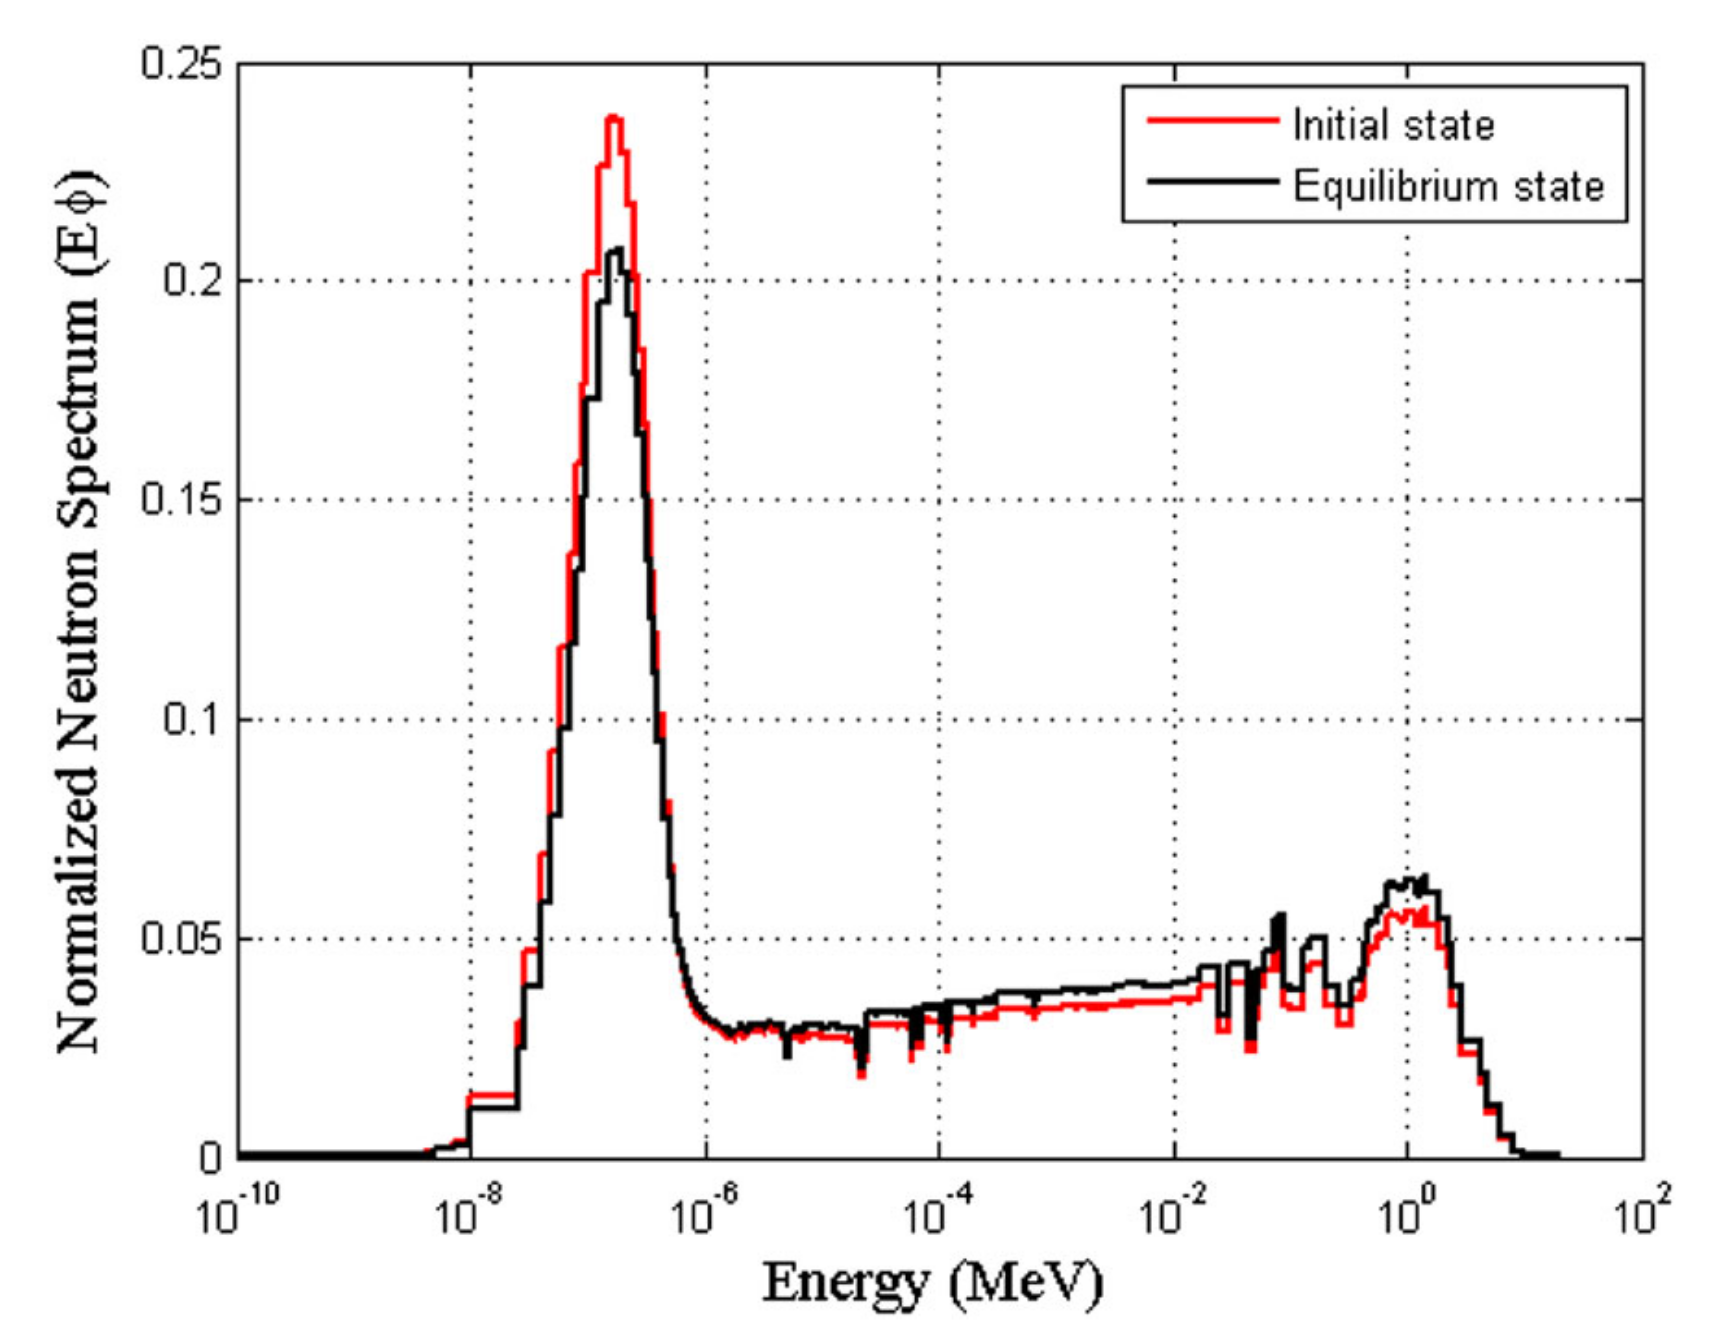
\includegraphics[width=0.5\linewidth]{figs/ch2/msbr_spectrum-park.png}
        \label{fig:msbr_spectrum_sub2}

    }\\`
    \subfloat[][]{
        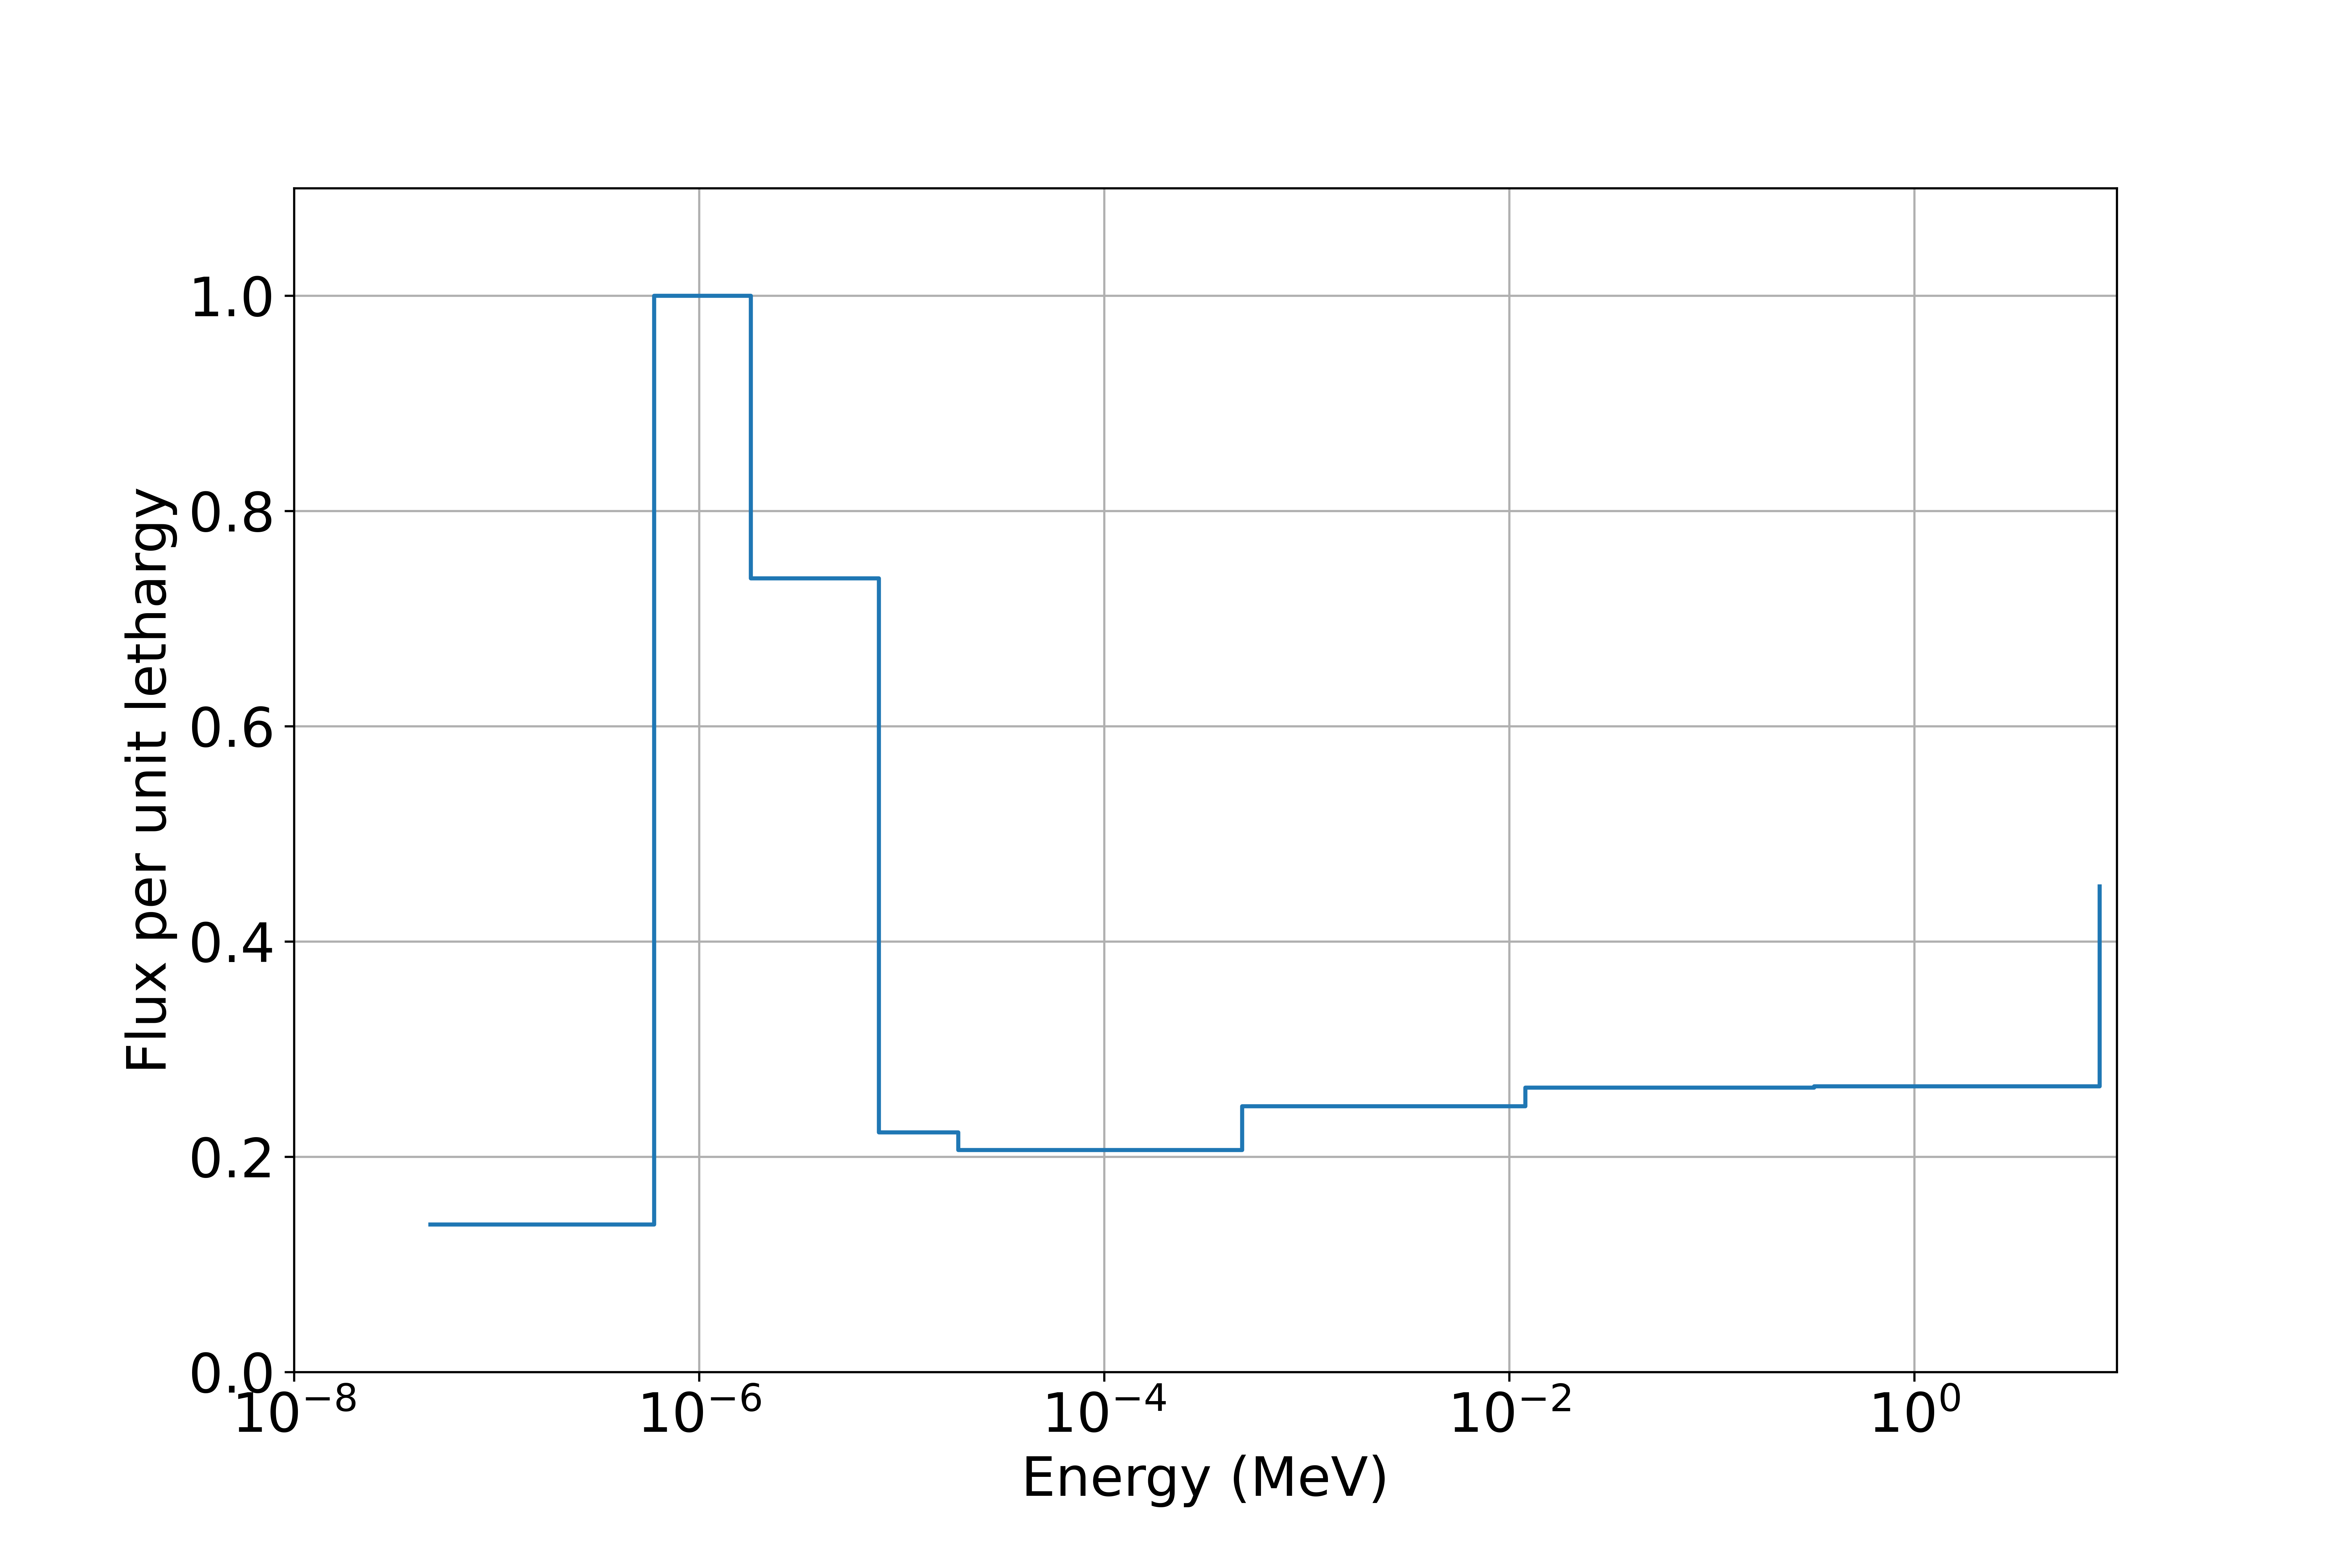
\includegraphics[width=0.6\linewidth]{figs/ch2/robertson_data.png}
        \label{fig:robertson_spectrum}
    }
    \caption[Side-by-side results of MSBR spectra between Ryhklevskii et al (2019) and Park et al (2015)]{
    \subref{fig:msbr_spectrum_sub1} Neutron flux energy spectrum at
    initial and equilibrium states normalized by unit lethargy. Reproduced
    from \cite{rykhlevskii_modeling_2019}; \subref{fig:msbr_spectrum_sub2}
    Neutron flux spectrum at initial and equilibrium states. Reproduced from
    \cite{park_whole_2015}; \subref{fig:robertson_spectrum} Neutron flux
    spectrum at the midplane of the MSBR design normalized by the peak flux. Made using data in Table B.2 in \cite{robertson_conceptual_1971}}
    \label{fig:msbr_spectrum_comp}
\end{figure}
% in andrei's paper he makes several claims about good agreement with the MSBR results in the Robertson report, but I have been unable to find said results in that report

%TODO: Compare some of the reported numbers for flux magnitude against andrei's figures in his papers/thesis

Rykhlevskii compared the TAP MSR results against an \Gls{ornl} technical report
on neutronic performance of the same reactor \cite{betzler_assessment_2017} using
identical cross section libraries and model parameters. Betzler et. al. used the
ChemTriton \cite{betzler_molten_2017} interface code that perfoms batch-wise
reprocessing using the \SCALE suite for coupled transport-depletion. ChemTriton
was extended to use the Shift \cite{davidson_nuclide_2018} monte carlo particle
transport tool for 3D neutron transport and depletion \footnote{at the time of
publication, Shift had not yet been incorporated into SCALE}. As seen in Figure
\ref{fig:tap-spectra}, neutron flux spectra results between the SaltProc and
ChemTriton simulations show qualitative agreement.

\begin{figure}[htpb]
    \centering
    \subfloat[][]{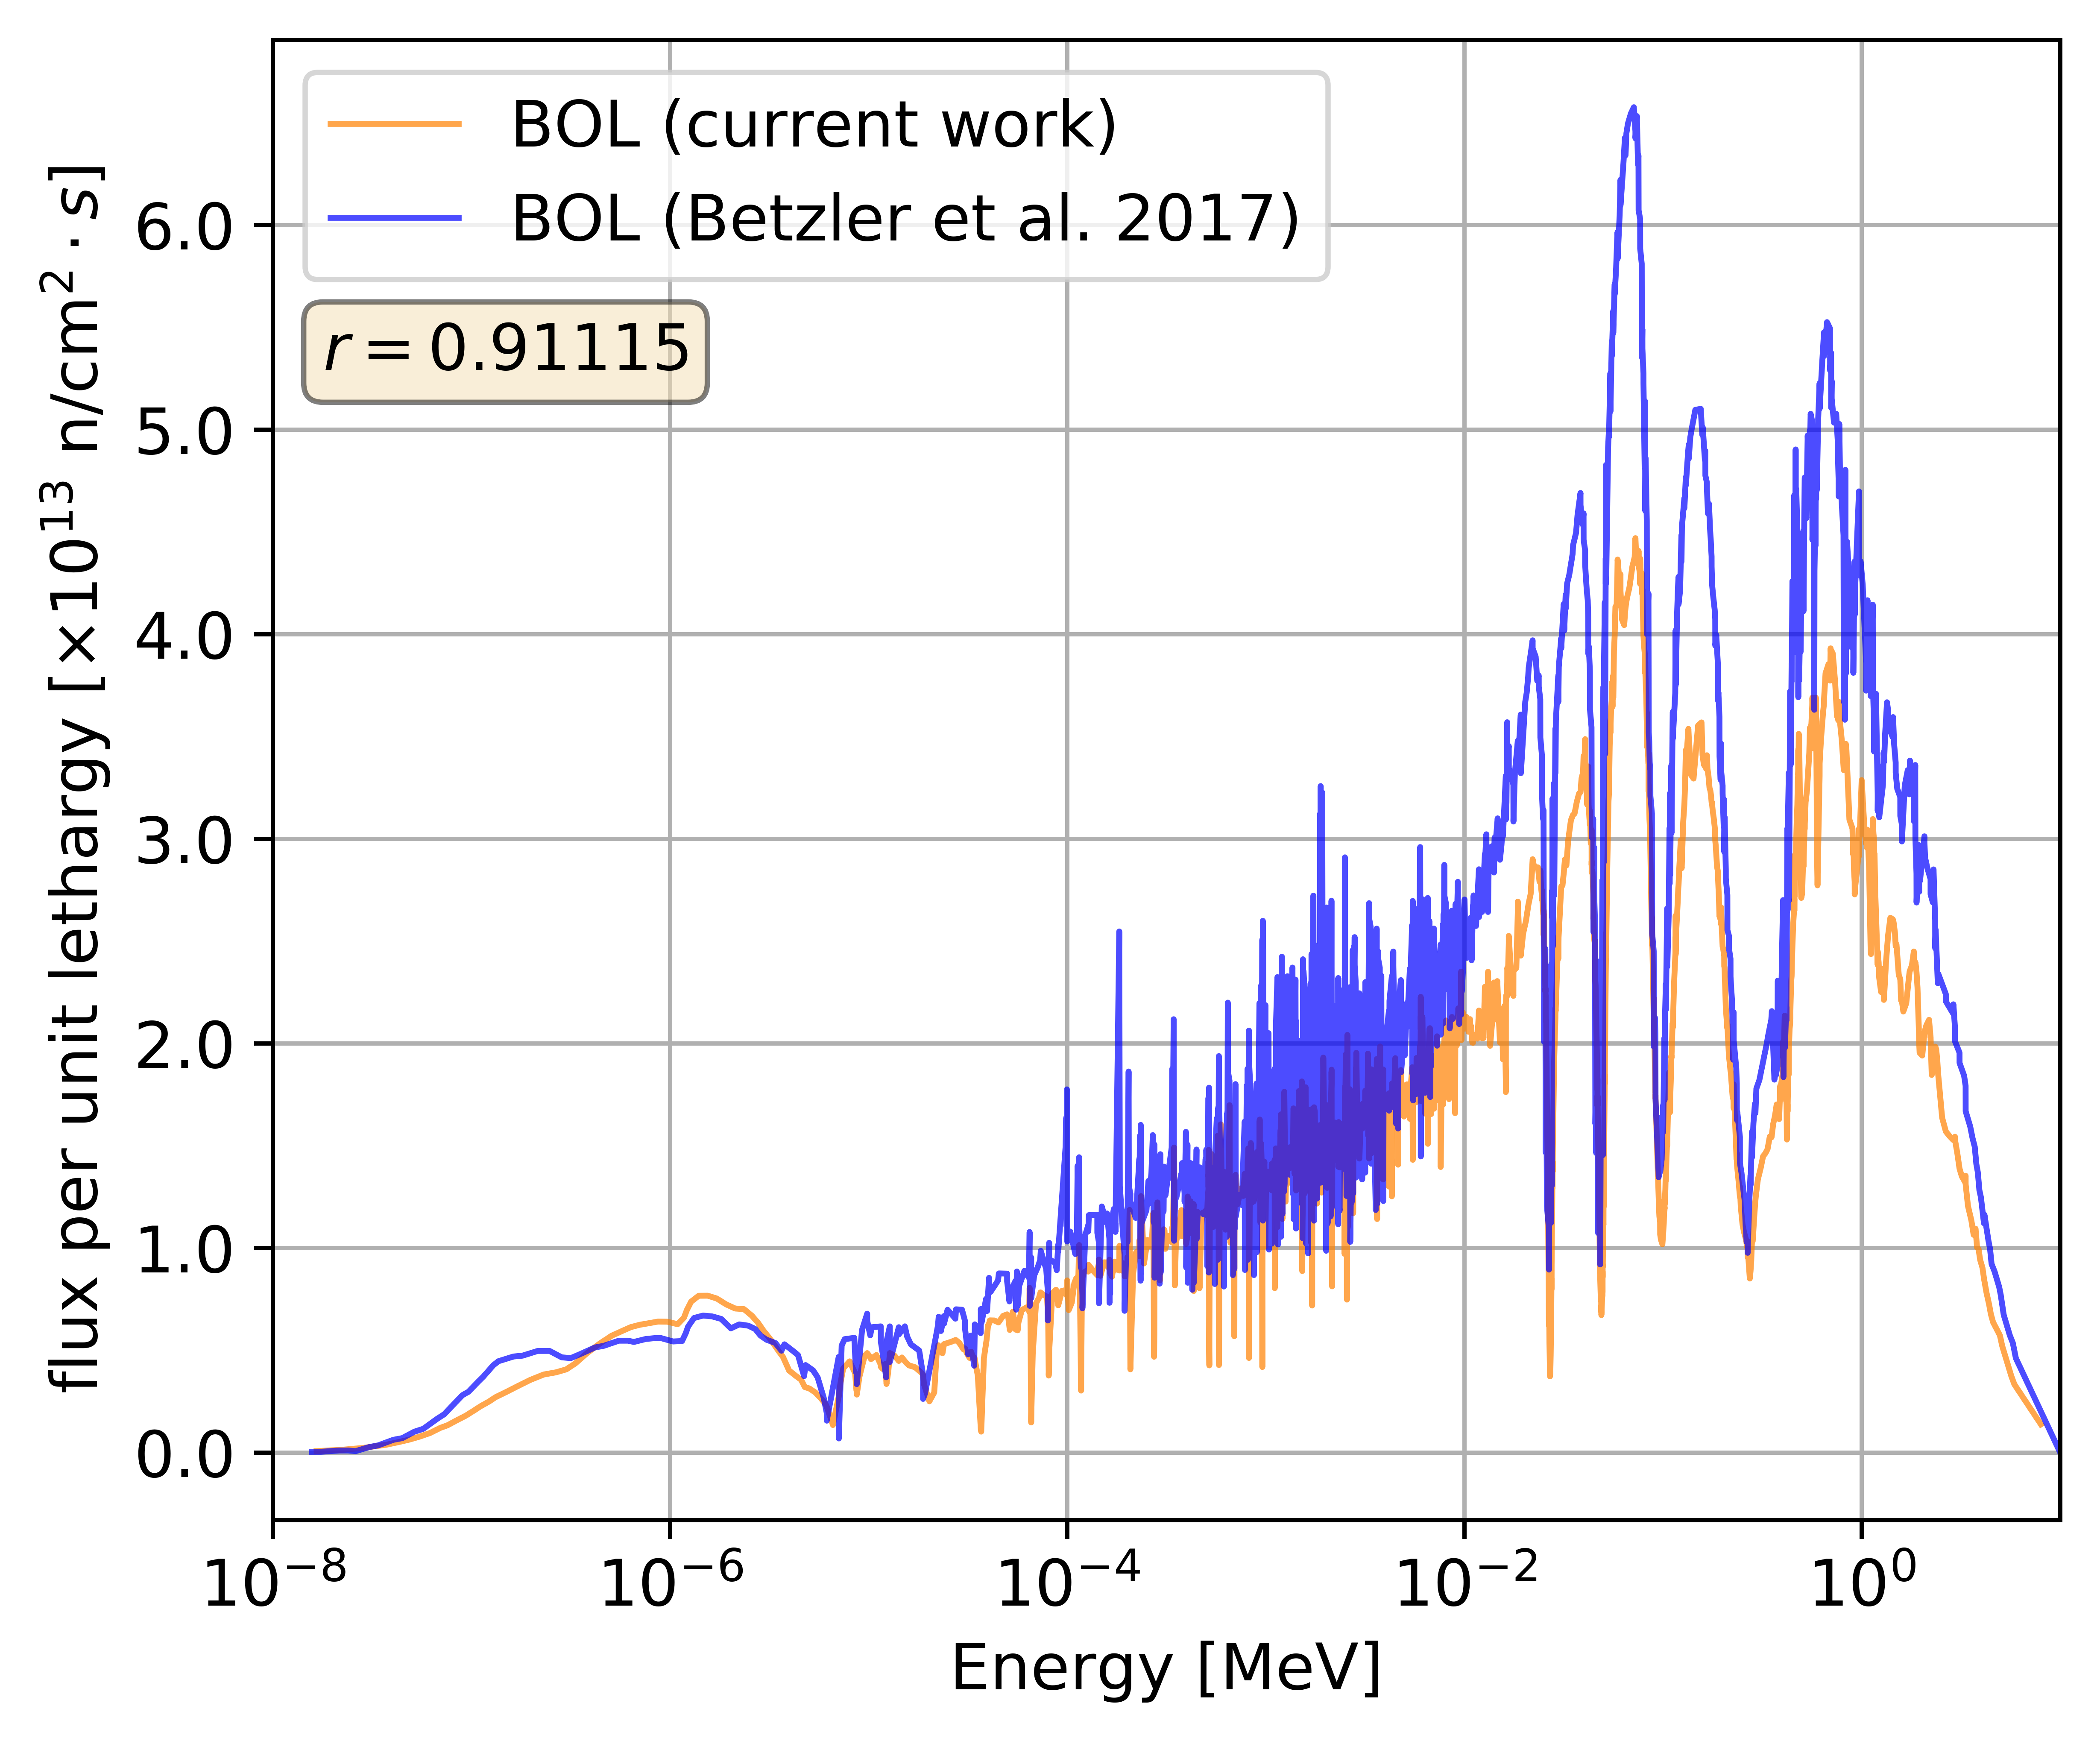
\includegraphics[width=0.5\linewidth]{figs/ch2/ben_spec_bol.png}
    \label{fig:tap-spectrum-bol}}
    \subfloat[][]{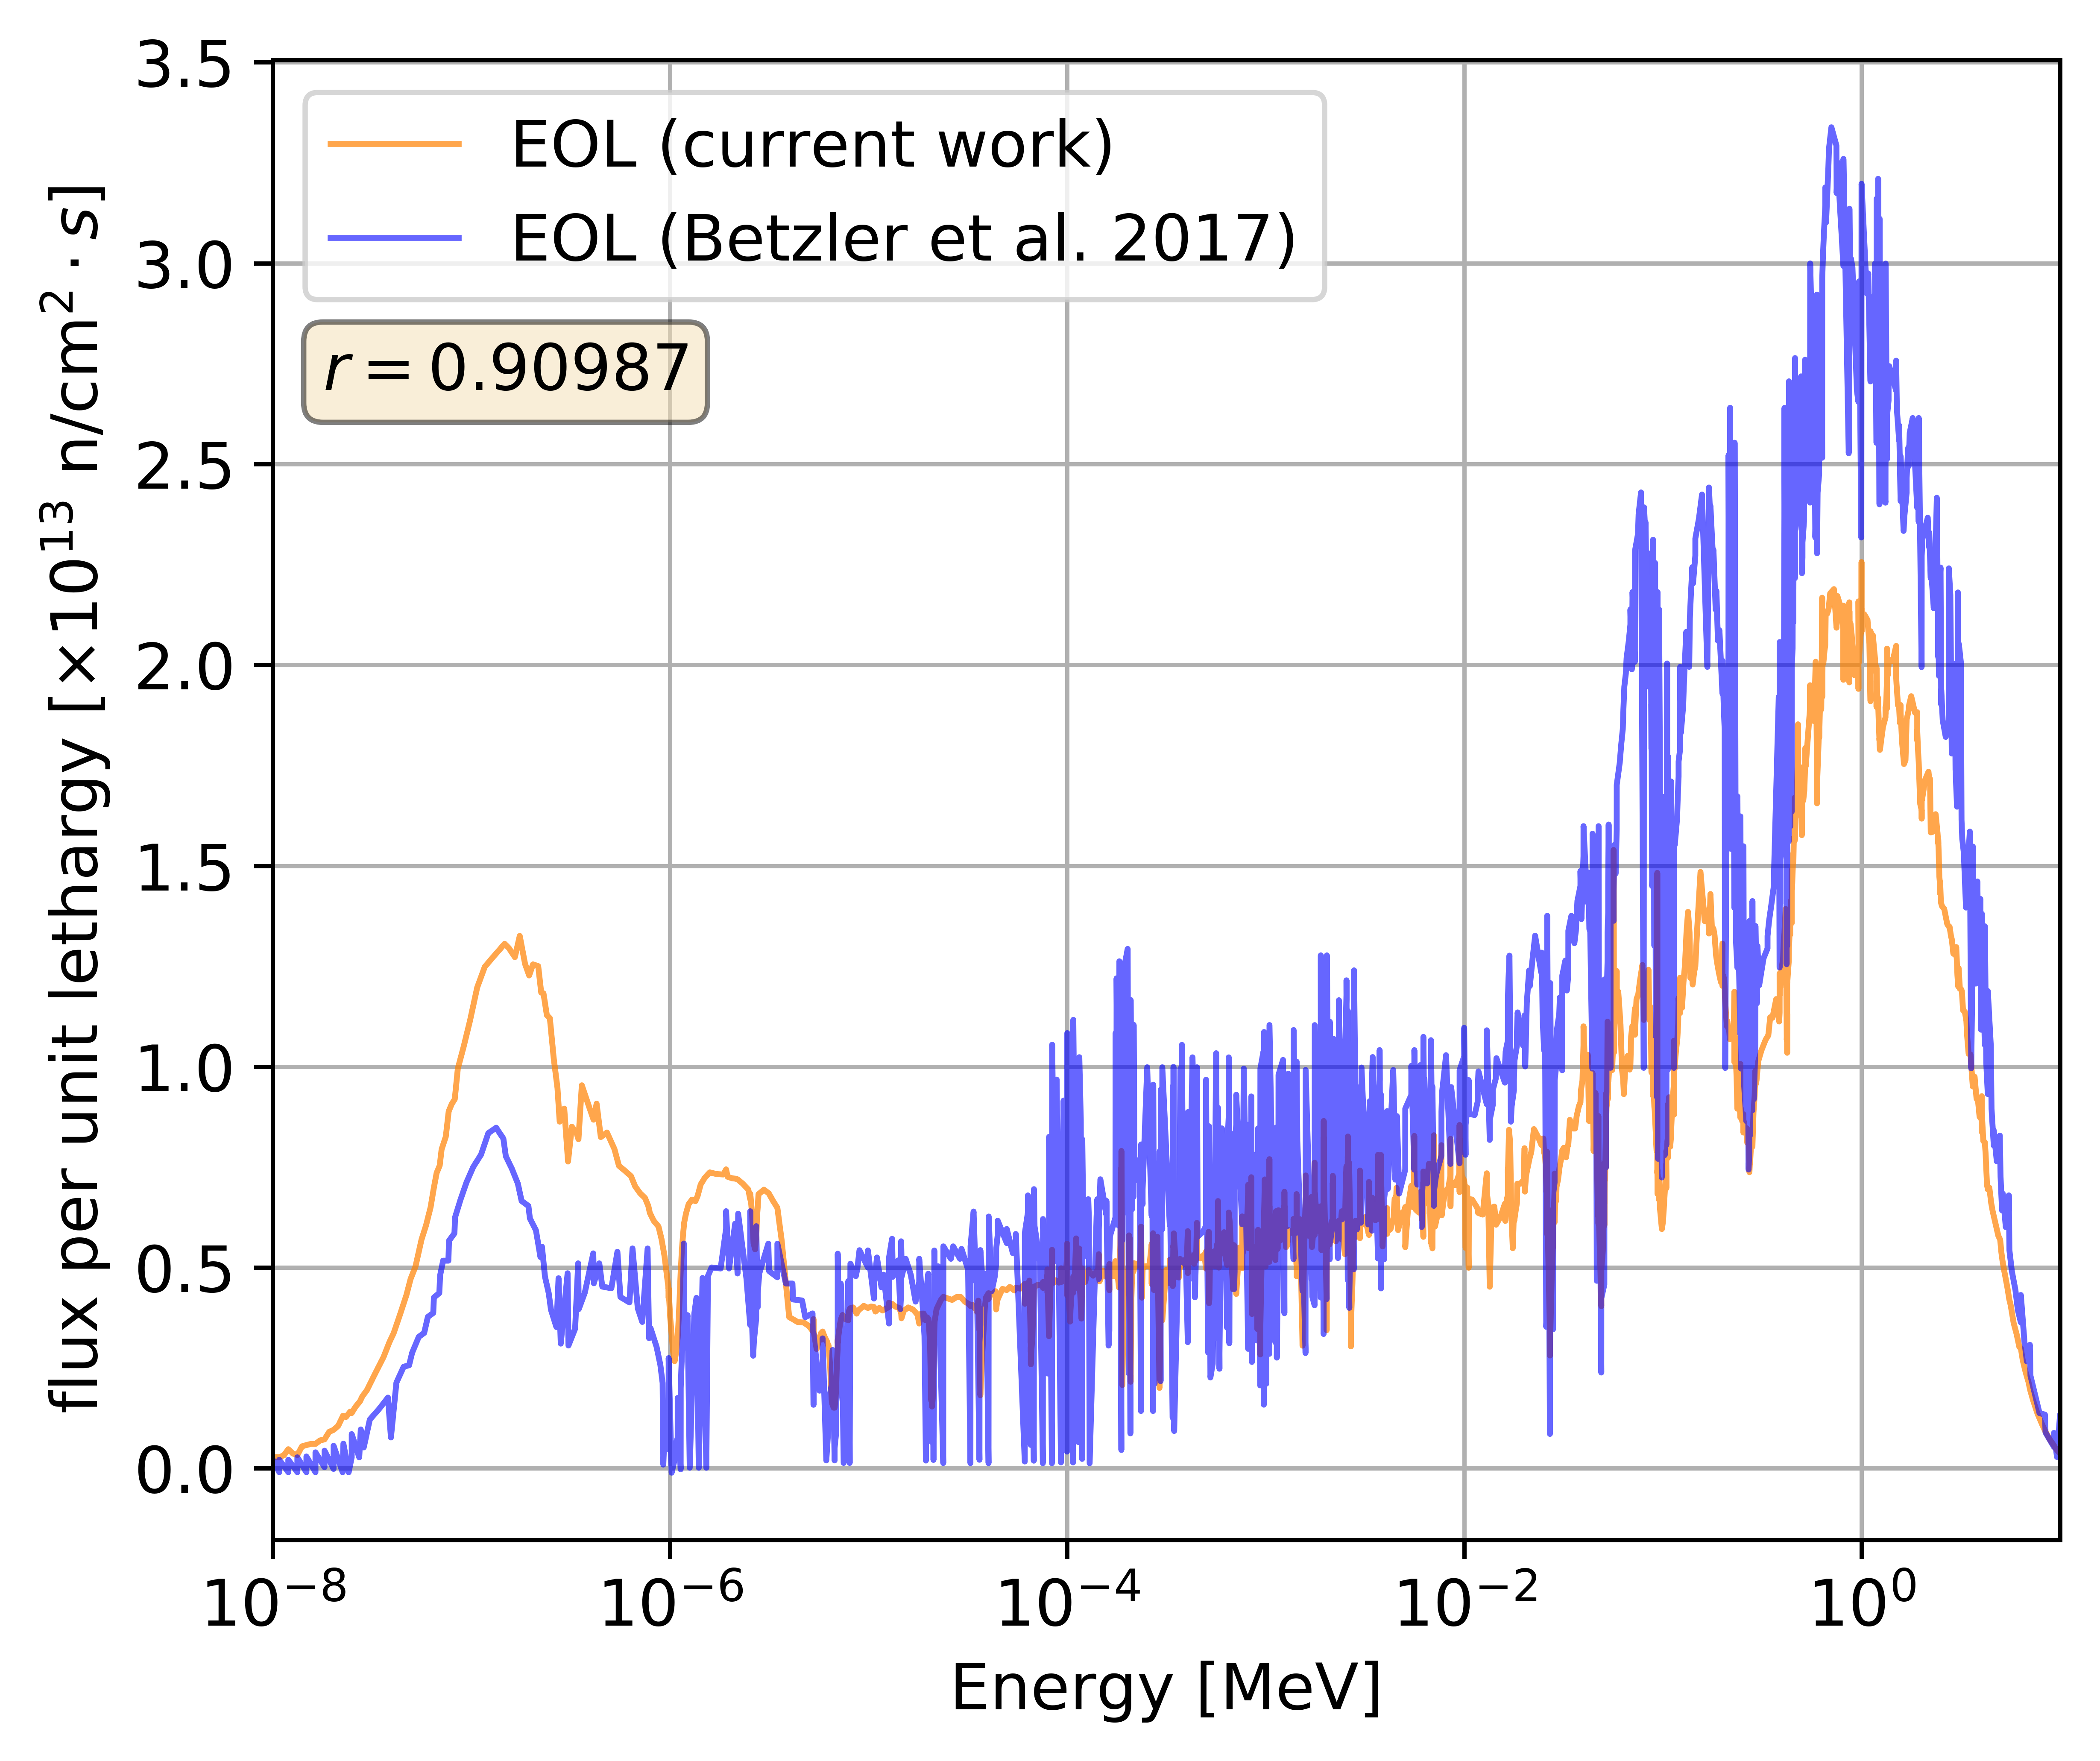
\includegraphics[width=0.5\linewidth]{figs/ch2/ben_spec_eol.png}
    \label{fig:tap-spectrum-eol}}
    \caption[Comparative results of TAP MSR flux spectra at BOL and EOL]{
        Comparative results of TAP MSR flux spectra at BOL and EOL:
        \subref{fig:tap-spectrum-bol} BOL;
        \subref{fig:tap-spectrum-eol} EOL;
        Both figures reproduced from \cite{rykhlevskii_fuel_2020}
    }
    \label{fig:tap-spectra}
\end{figure}

While \SaltProc has not been compared to \SCALE or \ADDER, these results verify
that \SaltProc produces results that are comparable to those of similar tools.


\subsection{Practical differences in continuous and batch-wise reprocessing}
We defined continuous and batch-wise reprocessing and discussed their
theoretical differences in in Section \ref{sec:msr_codes}. There are also some
practical implications on problem setup and results between these two methods.
Betzler, et. al. (2019) \cite{betzler_molten_2019} performed a code-to-code
comparsion between new functionality added to the \ORIGEN and \SCALE/\TRITON codes
for simulating depletion in \Gls{msr}s with continuous reprocessing, and the
older \ChemTriton \cite{betzler_molten_2017} interface code that performs
batch-wise reprocessing using the \SCALE suite for coupled transport-depletion.
They found that the two reprocessing schemes generally produced similar results
with the following caveats:
\begin{enumerate}
    \item $k_{\infty}$ for batch-wise reprocessing trends slightly lower than  continuous reprocessing. The authors claim this is due to \SCALE's {\it middlestep depletion method}. 
    \item The batch-wise method generally results in higher concentrations of nuclides. Notably, nuclides with short half lives, like \ce{^{135}Xe}, trends significantly higher in batch-wise reprocessing.
\end{enumerate}


\section{Differences between Serpent2 and OpenMC}
\label{sec:serpent-openmc-diff}
As mentioned in Section \ref{sec:objectives}, a major objective of this thesis
is to implement support for \OpenMC's \verb.deplete. module. In this context,
I would like to discuss some of the differences between \OpenMC and \SerpentTWO.
The most in-depth discussion of these differences that I have found are in
\cite{romano_depletion_2021}. I have tabulated the differences discussed in that
paper below.
\begin{table}[htpb] 
    \centering 
    \caption{Differences between \OpenMC and \SerpentTWO} 
    \label{tab:mc_code_diffs}
    \begin{tabulary}{\linewidth}{|C|C|C|} 
        \hline
        Metric & \OpenMC & \SerpentTWO \\ 
        \hline 
        Access & Open source, hosted on GitHub & Export controlled, code distributed by RSICC (USA), OECD/NEA\\
        \hline
        User interface & Python API & Manual writing of geometry, material, and settings files\\
        \hline 
        Handling of cross sections in between library temperatures & interpolation between neighboring temperatures & target motion-sampling \cite{viitanen_explicit_2012}\\
        \hline 
        Default matrix exponential solver & IPF CRAM-48 & PDF CRAM-14 \\
        \hline
        Cross section file format & HDF5 & ACE \\
        \hline
        S$(\alpha, \beta)$ representation & continuous & tabulated \\
        \hline
        Depletion data source & ENDF decay and fission product yield sublibraries & depletion chain XML file\\
        \hline
        Default method to calculate fission product yields & various & energy-weighted average interpolation \cite{kunchev_energy-dependent_2019}\\
        \hline
    \end{tabulary}
\end{table}
As mentioned earlier, Romano found good agreement between \OpenMC depletion
results and \SerpentTWO depletion results. I will now briefly discuss these
results in more detail.

\OpenMC's depletion module contains functions to create a depletion chain from
user-provided data. Romano et al used three different depletion chains in their
study \cite{romano_depletion_2021}:
\begin{enumerate}
    \item A full depletion chain that contains data from ever neutron, decay
        and fission product yield sublibray file in the ENDF/B-VII.1 library.
    \item A reduced depletion chain that finds all potential products from the
        nuclear reactions based on a set of starting nuclides to reduce the
        size of the depletion matrix.
    \item A depletion chain based on the VERA depletion benchmark
        specifictation \cite{kim_specification_2015}, referred to as the CASL
        depletion chain by Romano et al \cite{romano_depletion_2021}.
\end{enumerate}
\SerpentTWO allows users to select same data using the appropriate ``set''
cards, however does not include a method to reduce the depletion chain or
modify a depletion chain directly, meaning that the CASL depletion chain cannot
be used with the version of \SerpentTWO used in \cite{romano_depletion_2021}
(2.1.31).

\OpenMC's depletion module also contains various methods for obtaining reaction
rates, calculating power normalization of reaction rates, and selecting fission
product yields. Romano et al used two methods  for selecting the fission
product yields \cite{romano_depletion_2021}. One is to simply use fission product
yields at thermal energy, and the other is analagous to the method use in
ORIGEN \cite{gauld_isotopic_2011} where the average energy of neutrons causing
fission determines the evaluation point for linearly interpolated fission
product yields.

The three different depletion chains and two different fission product yield
methods composed the five\footnote{There was only one case using the reduced
depeltion chain as it was expected to produce identical results to the full
depletion chain} simulation cases for depletion on a PWR pincell model.

\begin{figure}[htpb]
    \centering
    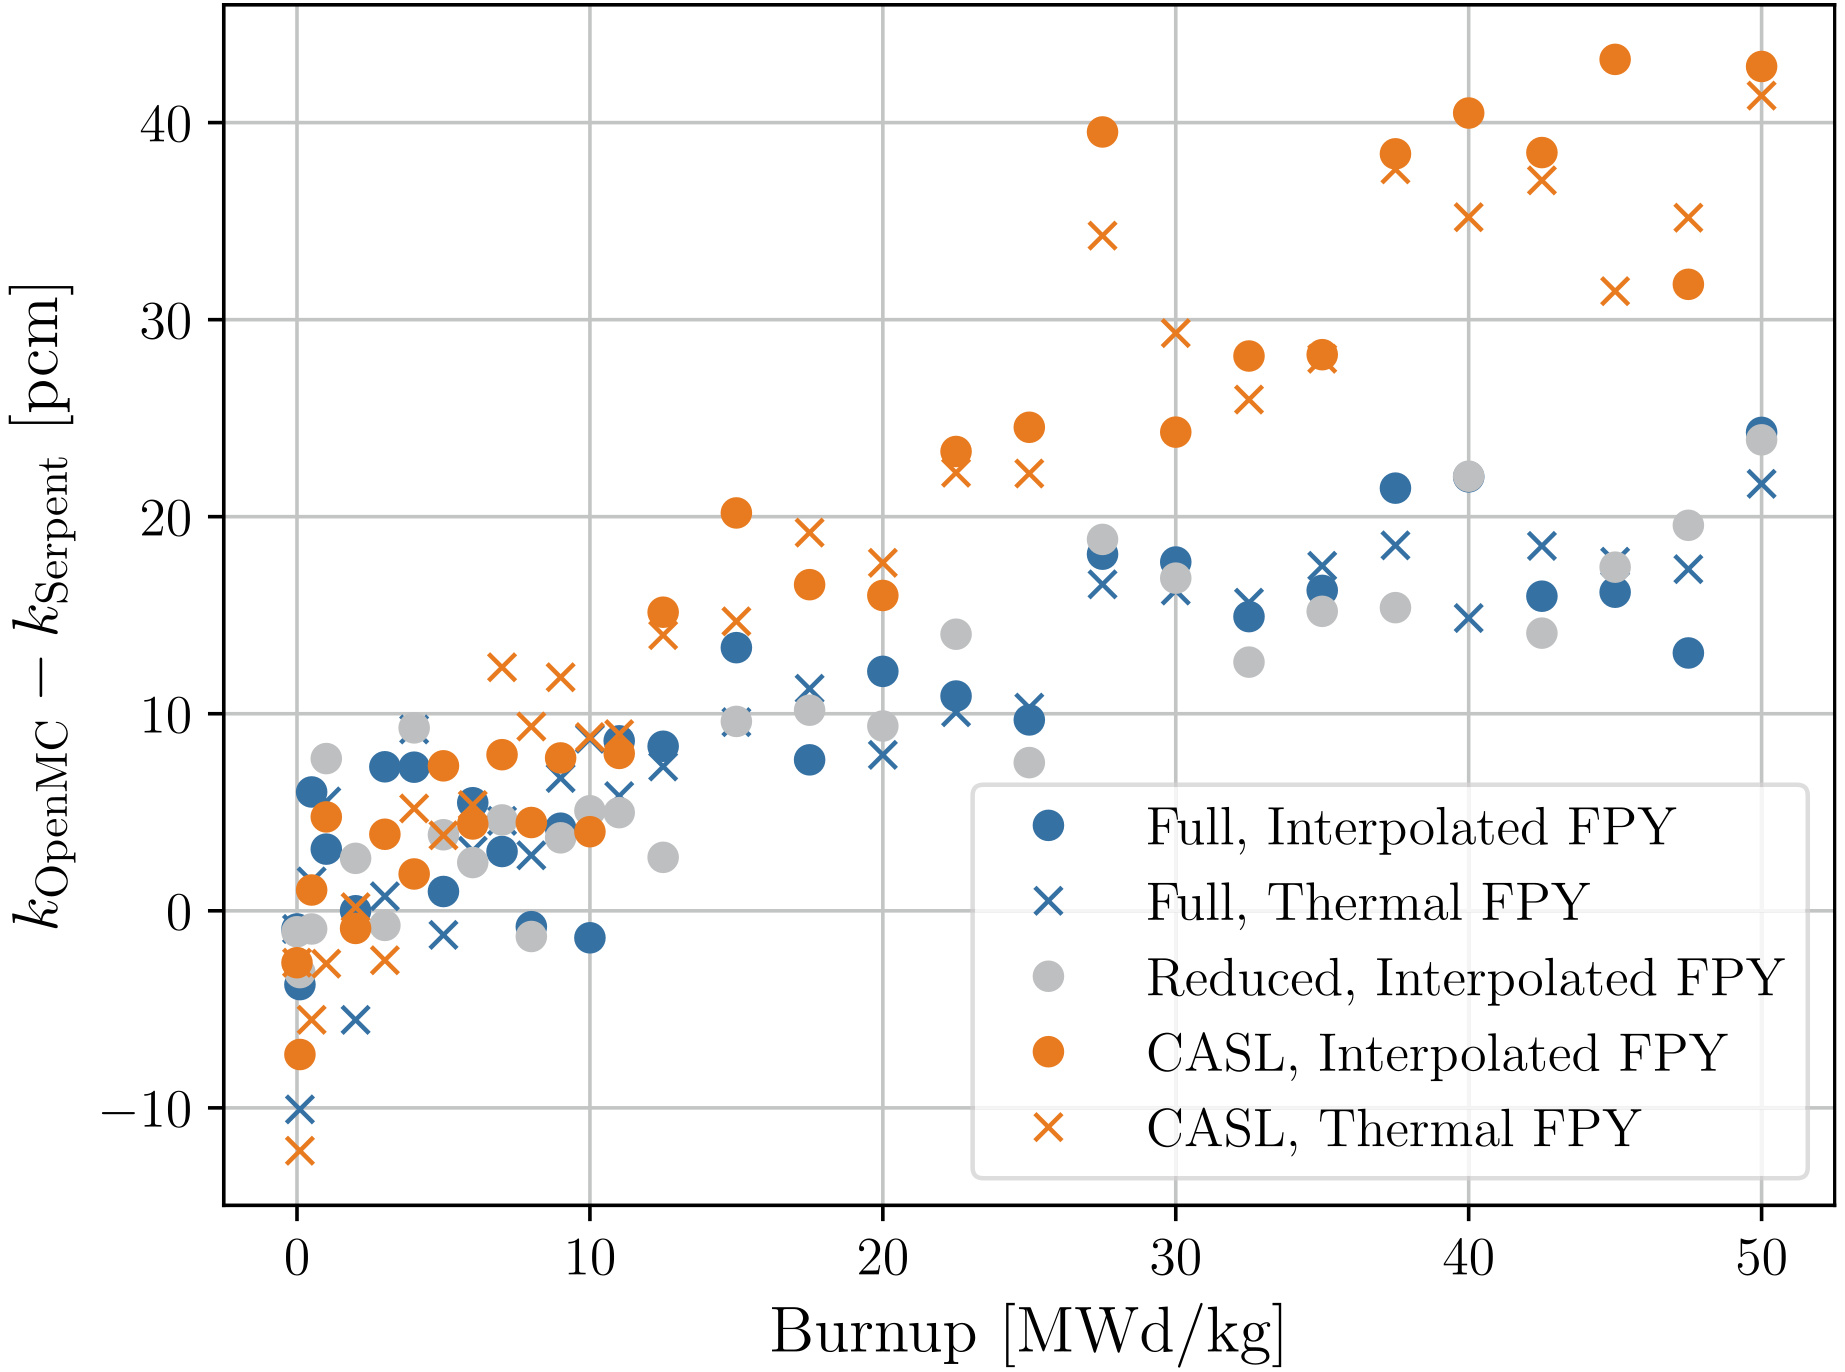
\includegraphics[width=0.5\textwidth]{figs/ch2/serpent_openmc_keff.png}
    \caption[Difference in the effective multiplication factor, $k_\text{eff}$
    between OpenMC and Serpent for the PWR pincell model.]{Difference in the
    effective multiplication factor, $k_\text{eff}$ between OpenMC and Serpent
    for the PWR pincell model. While not shown, the one standard deviation
    uncertainty in the difference is about 3.5 pcm. Reproduced from Figure 2 in
    \cite{romano_depletion_2021}}
    \label{fig:pwr-serpent-openmc-keff}
\end{figure}

Figure \ref{fig:pwr-serpent-openmc-keff} shows the differences in $k_\text{eff}$
for all five cases. The difference at the end of the depletion simualation is
around 20pcm for the full chain and around 40pcm for the CASL chain. The
reduced chain is more or less identical to the full chain with some outlying
points in time. As expected, the smallest differences between the calculated
$k_\text{eff}$ in \SerpentTWO and \OpenMC depletion simultions occur when the
depeletion chains used are identical.

\begin{figure}[htpb]
    \centering
    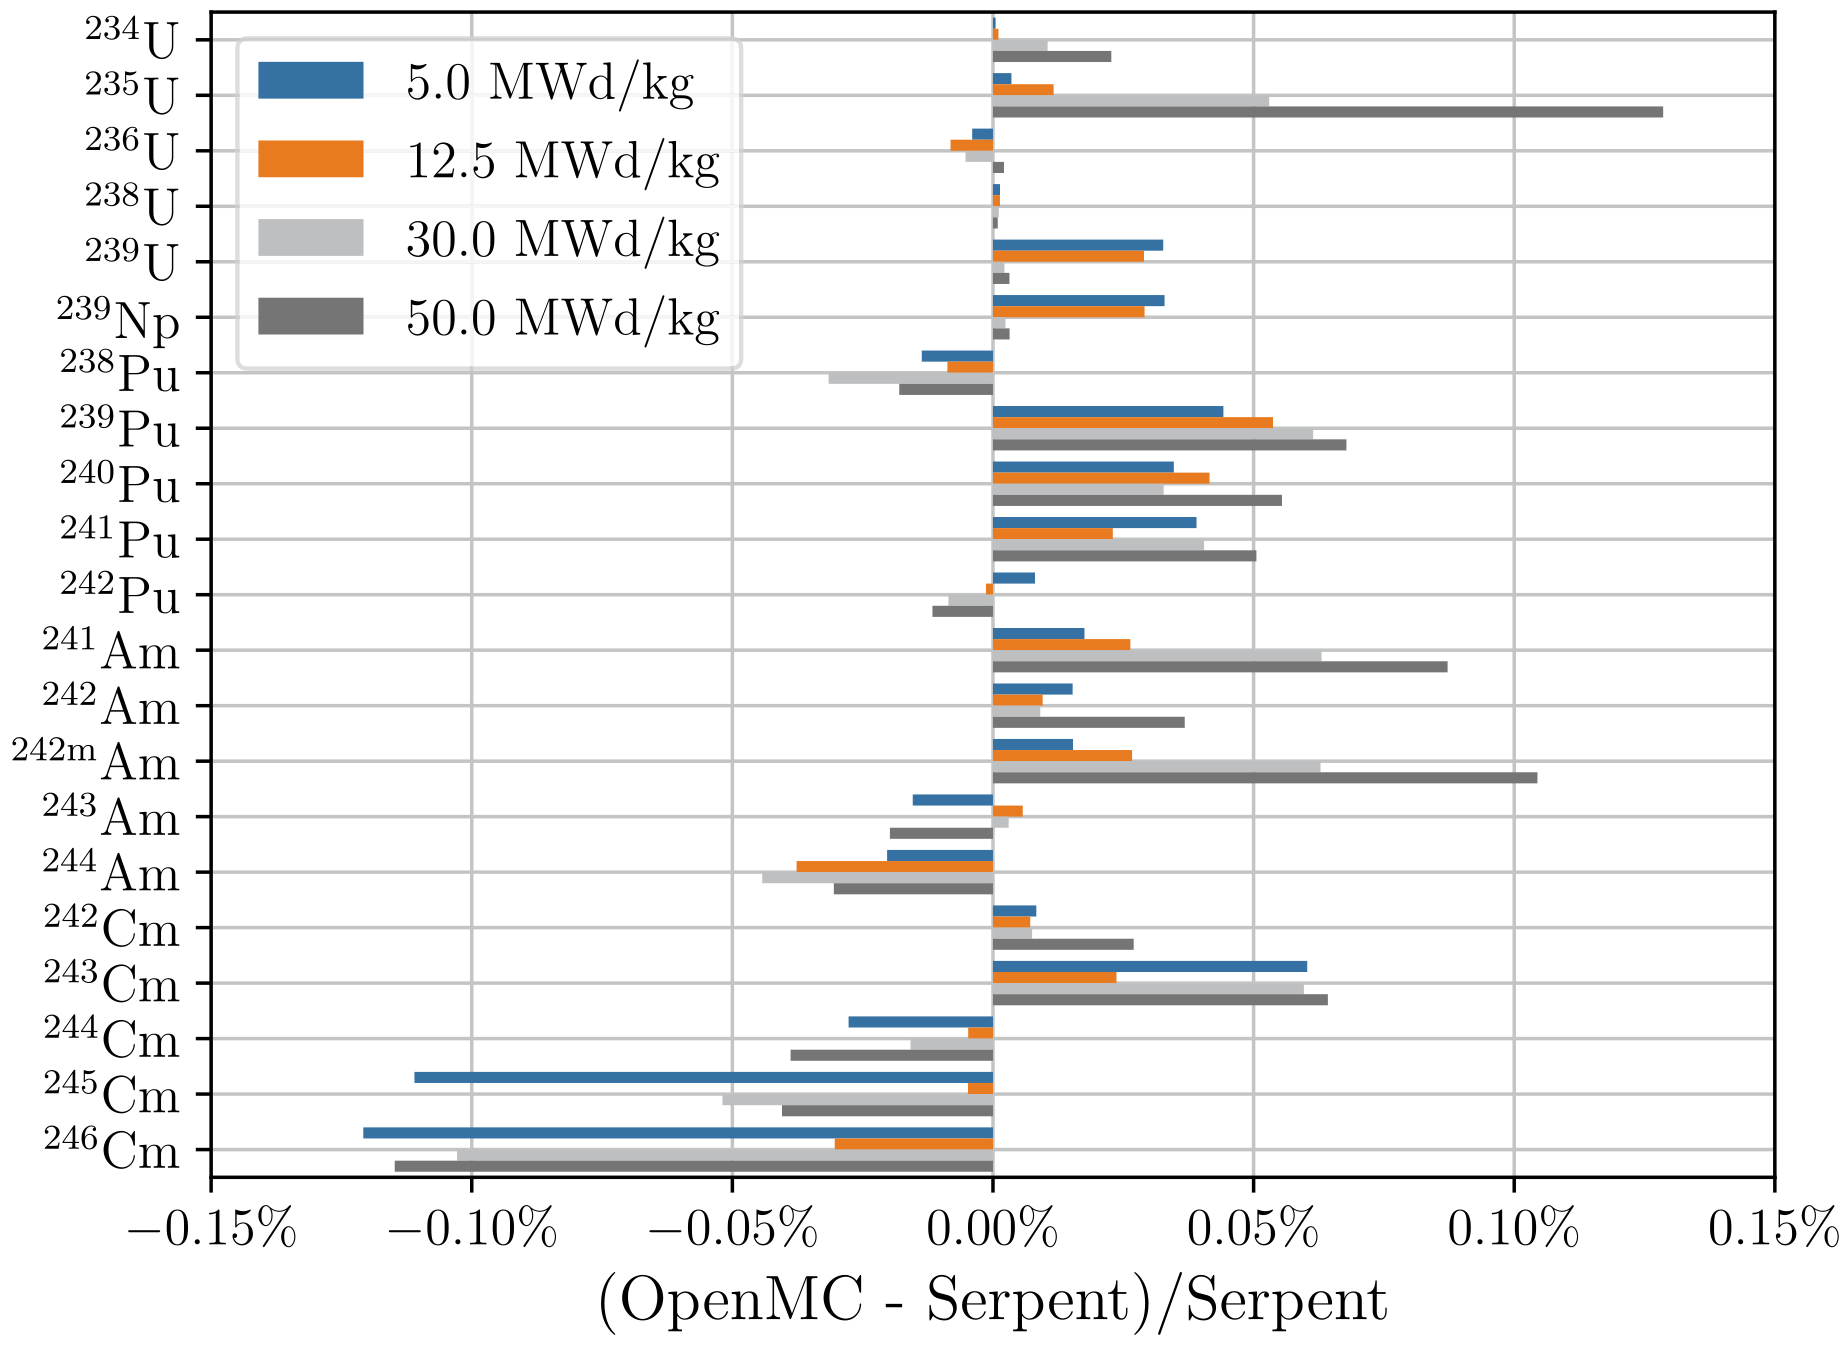
\includegraphics[width=0.5\textwidth]{figs/ch2/serpent_openmc_actinides.png}
    \caption[Relative difference in actinide concentrations bewteen OpenMC and
    Serpent for the PWR pincell model.]{Relative difference in actinide
    concentrations between OpenMC and Serpent for the PWR pincell model at 5,
    12.5, 30, and 50 MWd/kg using the full depletion chain. Reproduced from
    Figure 3 in \cite{romano_depletion_2021}}
    \label{fig:pwr-serpent-openmc-actinides}
\end{figure}

Figure \ref{fig:pwr-serpent-openmc-actinides} shows the relative difference in
actinide concentrations using the full depletion chain. Most of the differences
are less than 0.1\% and all are within 0.15\%. 

\begin{figure}[htpb]
    \centering
    \subfloat[][]{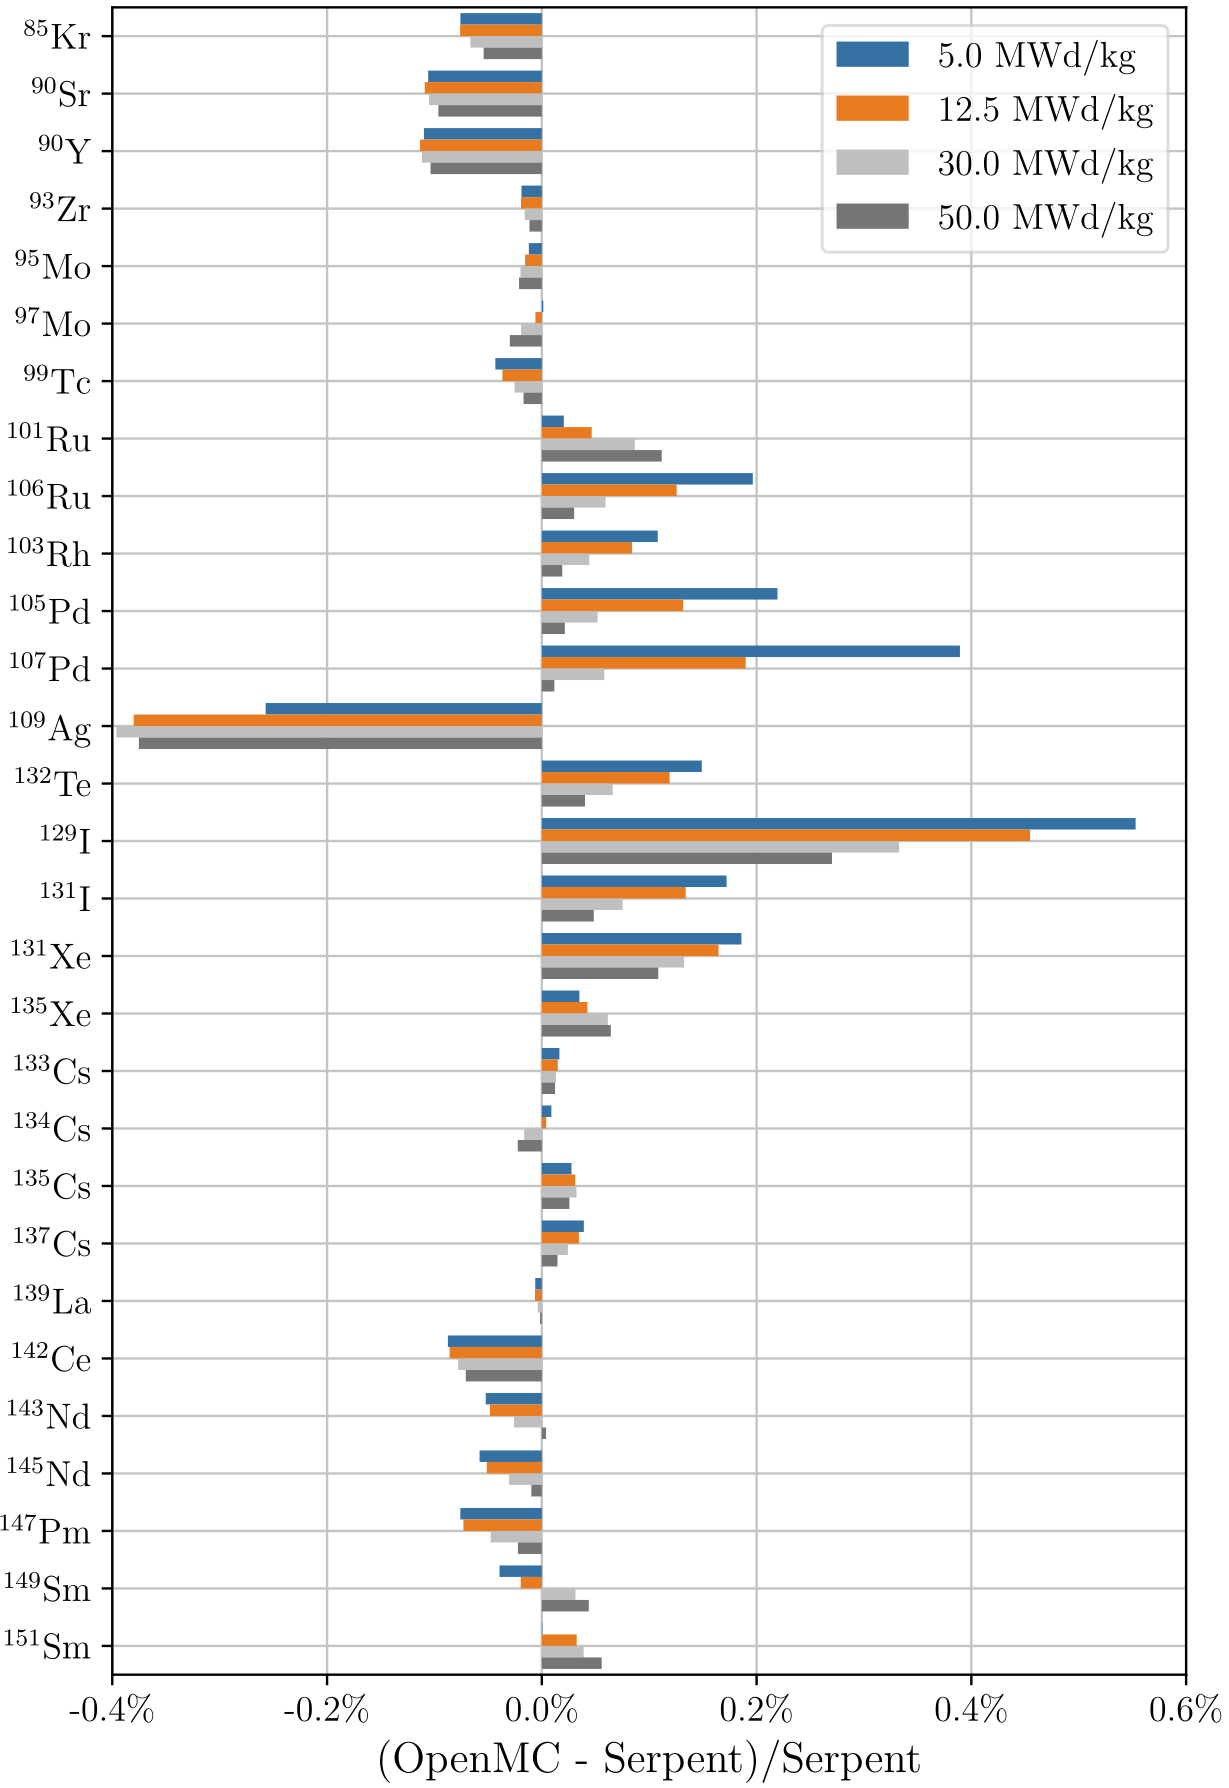
\includegraphics[width=0.5\linewidth]{figs/ch2/serpent_openmc_fp_interpolated.png}
    \label{fig:serpent-openmc-fp-interp}}
    \subfloat[][]{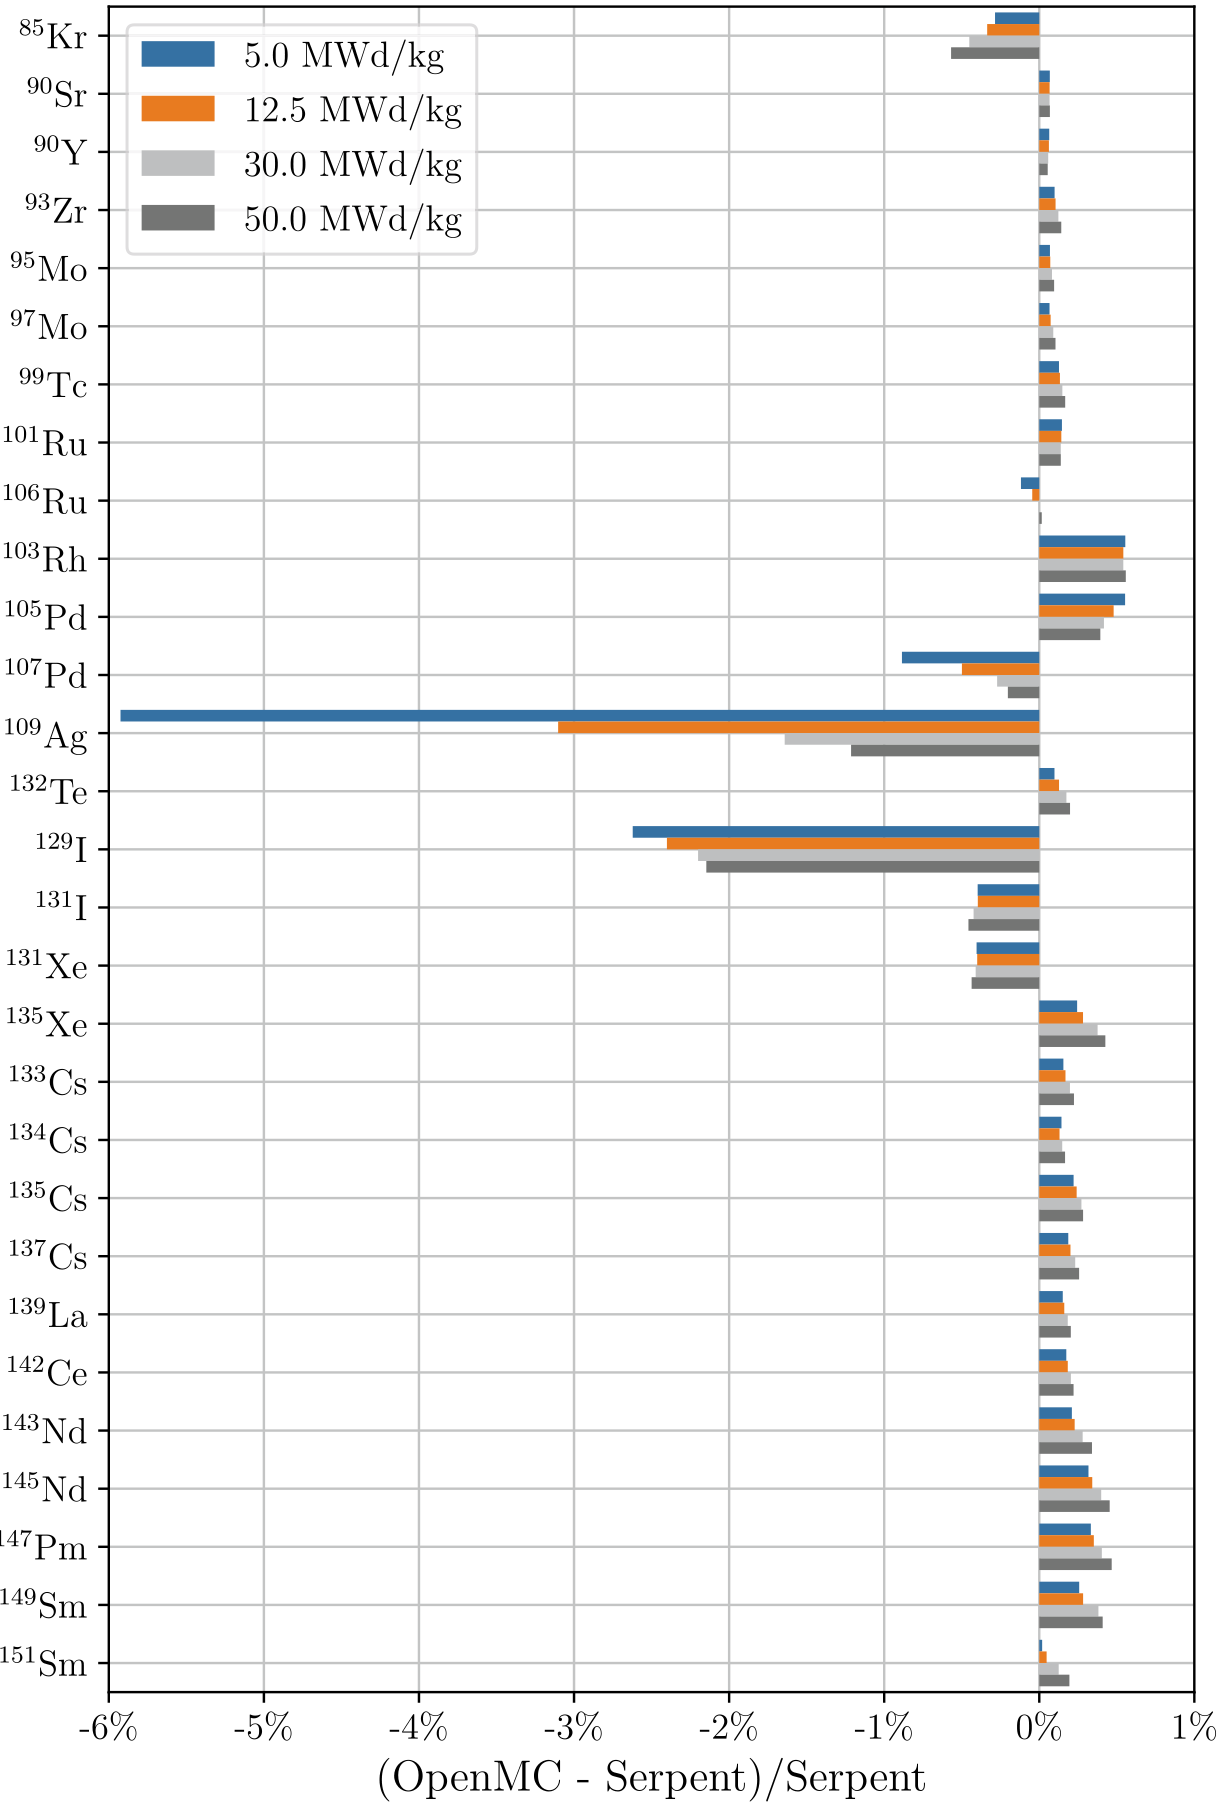
\includegraphics[width=0.5\linewidth]{figs/ch2/serpent_openmc_fp_thermal.png}
    \label{fig:serpent-openmc-fp-therm}}
    \caption[Relative difference in fission product concentrations between
    OpenMC and Serpent for the PWR pincell model]{Relative difference in fission
    product concentrations between OpenMC and Serpent for the PWR pincell model
    at 5, 12.5, 30, and 50 MWd/kg using the full depletion chain and:
    \subref{fig:serpent-openmc-fp-interp} interpolated fission product yields;
    \subref{fig:serpent-openmc-fp-therm} thermal fission product yields.
    Both figures reproduced from \cite{romano_depletion_2021}}
    \label{fig:pwr-serpent-openmc-fp}
\end{figure}

Figures \ref{fig:serpent-openmc-fp-interp} and
\ref{fig:serpent-openmc-fp-therm} show the relative difference in fission
product concentrations using interpolated and thermal fission product yields,
respectively. Interpolated fission yields give the smallest differences, with
most differences being less that 0.2\% and all differences bein within 0.6\%,
wheras thermal fission yields bump up the errors by an order of magnitude. This
shows us that using interpolated fission yields for \OpenMC depletion
simulations will give us very good agreement with the \SerpentTWO depletion
results.

Romano et al also compared depletion performance between \OpenMC and
\SerpentTWO on a model of the \Gls{sfr} \cite{oecd_benchmark_2016}, which is a
fast reactor design. Compared to the PWR pincell study, the results of this
study showed similar trends and magnitudes in the time-dependent nuclide
concantrations with respect to whether or not the depletion settings and
depletion chains used were the same. The differences in $k_\text{eff}$ also
followed a similar trend as in the PWR pincell study, but with larger
magnitudes. This shows that \OpenMC and \SerpentTWO maintain good agreement for
depletion even on more complex geometries.

While these results are in good agreement, obtaining them took careful
consideration of settings and methods uses by each code. In addition to the
depletion settings and methods used by the codes,  Romano et al notes that one
must take careful consideration of the data and internal settings to get good
results between codes. Of note are the default energy release per fission of
\ce{^{235}U} used for power normalization and capture branching ratios. We
follow Romano's methodology to ensure data consistency in our comparative
study. The key features to consider:
\begin{itemize}
    \item Utilize identical cross-section libraries, depletion data, and capture branching ratios
    \item Use the same fission heating values.
\end{itemize}
We will discuss our procedure for ensuring data consistency in Chapter 4.
%% talk about saltproc in it's current state, the gaps that exist
%% lead into discussion about why it's important to add openmc 
%% capabilities to SaltProc. Also mention the differences in 
%% Serpent2 and OpenMC cross section handling and how this
%% adds capability to the SaltProc tool
